\documentclass[../../main.tex]{subfiles}
    
    \lstset{basicstyle=\small,
      showstringspaces=false,
      commentstyle=\color{black},
      keywordstyle=\color{blue}
    }

    \graphicspath{{images/Maschinentechnik/}{../../images/Maschinentechnik/}}

    \begin{document}
    \subsection{Konzeptentwicklung Maschinentechnik}
    Im Bereich Maschinentechnik des Projektes wird konkret auf die Thematik der Mechanik eingegangen. Die einzelnen Komponenten sind jedoch eng mit der Elektronik und der Informatik verknüpft. Die projektspezifische Mechanik wird in folgende drei Hauptgruppen unterteilt: Fahrwerk, Würfeltransport und Antrieb. In diesem Kapitel werden die mechanischen Lösungsvorschläge der definierten Teilfunktionen vorgestellt und bewertet. Der Morphologischer Kasten dient dabei als Grundlage der Lösungsfindung. Durch ihn wurden Varianten generiert, welche anschliessend mit definierten Bewertungskriterien in einer Nutzwertanalyse ausgewertet werden. Die zwei Varianten, welche den grössten Nutzwert aufweisen werden nochmals genauer beschrieben. Zusätzlich wird anhand der Vor- und Nachteile eine favorisierte Lösung für jede Problemstellung festgelegt. Das Komplette Dokument der Nutzwertanalyse der Mechanik ist im Anhang zu finden.

    \subsubsection{Fahrwerk}
    \textbf{Kurvenfahrt}\\
    Das Ziel der Kurvenfahrt ist es, sie möglichst schnell abzufahren, ohne dabei aus den Gleisen zu fallen. Anhand der Nutzwertanalyse haben sich die zwei besten Varianten Schwenker und tiefer Schwerpunkt für die Konzeptbildung herauskristallisiert und werden nun genauer beschrieben (siehe Abbildung \ref{fig:kurvenfahrt}).

    \begin{figure}[H] %Nutzwertanalyse Kurvenfahrt
        \centering
        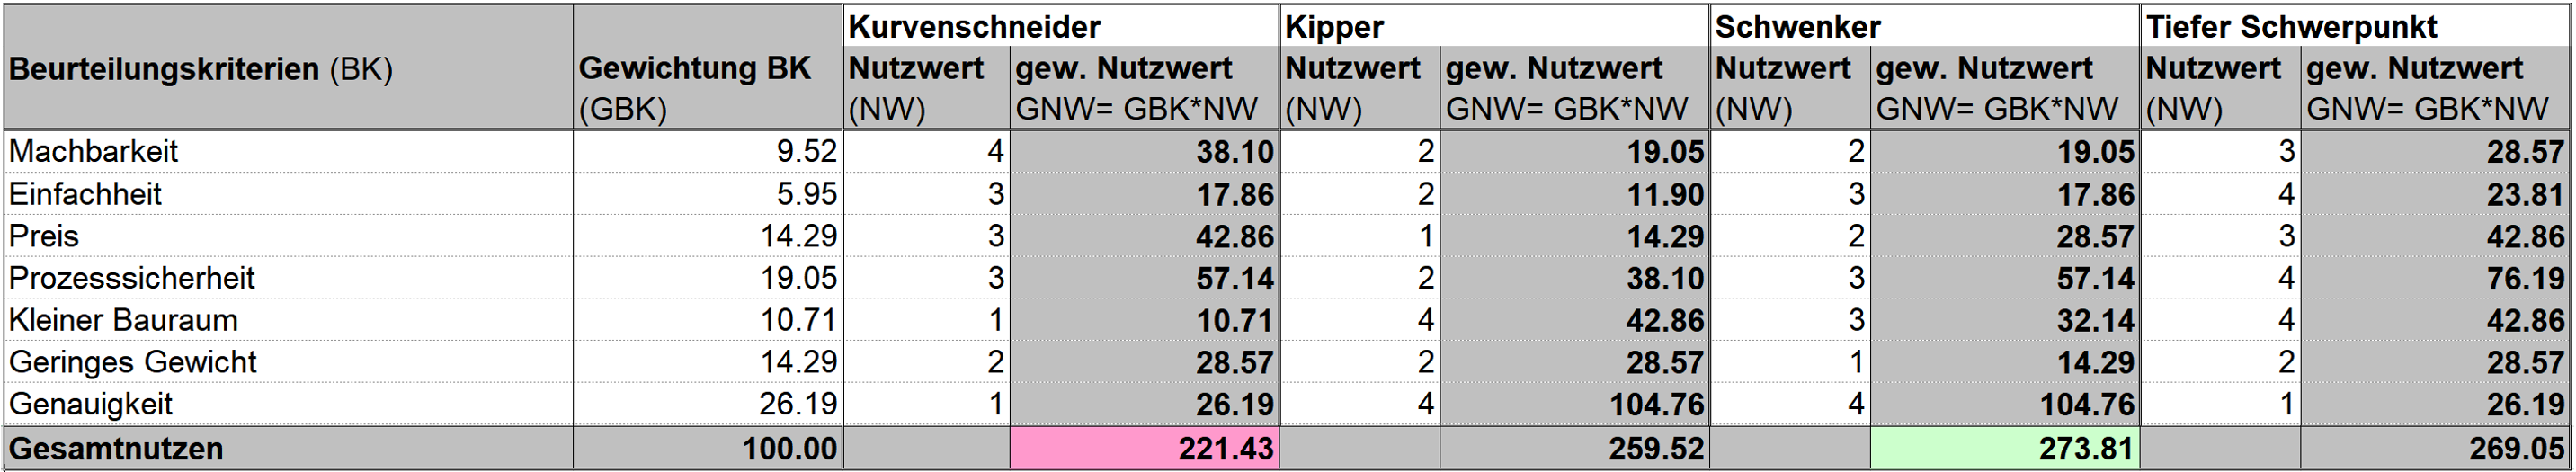
\includegraphics[width=1\textwidth]{Kurvenfahrt}
        \caption{Nutzwertanalyse Kurvenfahrt}
        \label{fig:kurvenfahrt}
    \end{figure}
    
    \textbf{Schwenker}\\
    Der Schwenker in Abbildung \ref{fig:schwenker} ist eine Lösungsvariante, bei welcher eine Masse quer über den Zugwagen beweglich und steuerbar angebracht ist. Damit soll gewährleistet werden, dass der Massenschwerpunkt in einer Kurve zum Radiusmittelpunkt hin verschoben werden und somit die Zentripetalkraft ausgeglichen werden kann. Zusätzlich kann der Schwenker ebenfalls für die Thematik des Greifens und Verschiebens des Würfels genutzt werden, denn dort wirken ebenfalls Momente quer auf den Zug. In der Tabelle \ref{tab:schwenker} sind die Vor- und Nachteile dieser Variante aufgelistet.
    
    \begin{figure}[H] % Skizze Schwenker
        \centering
        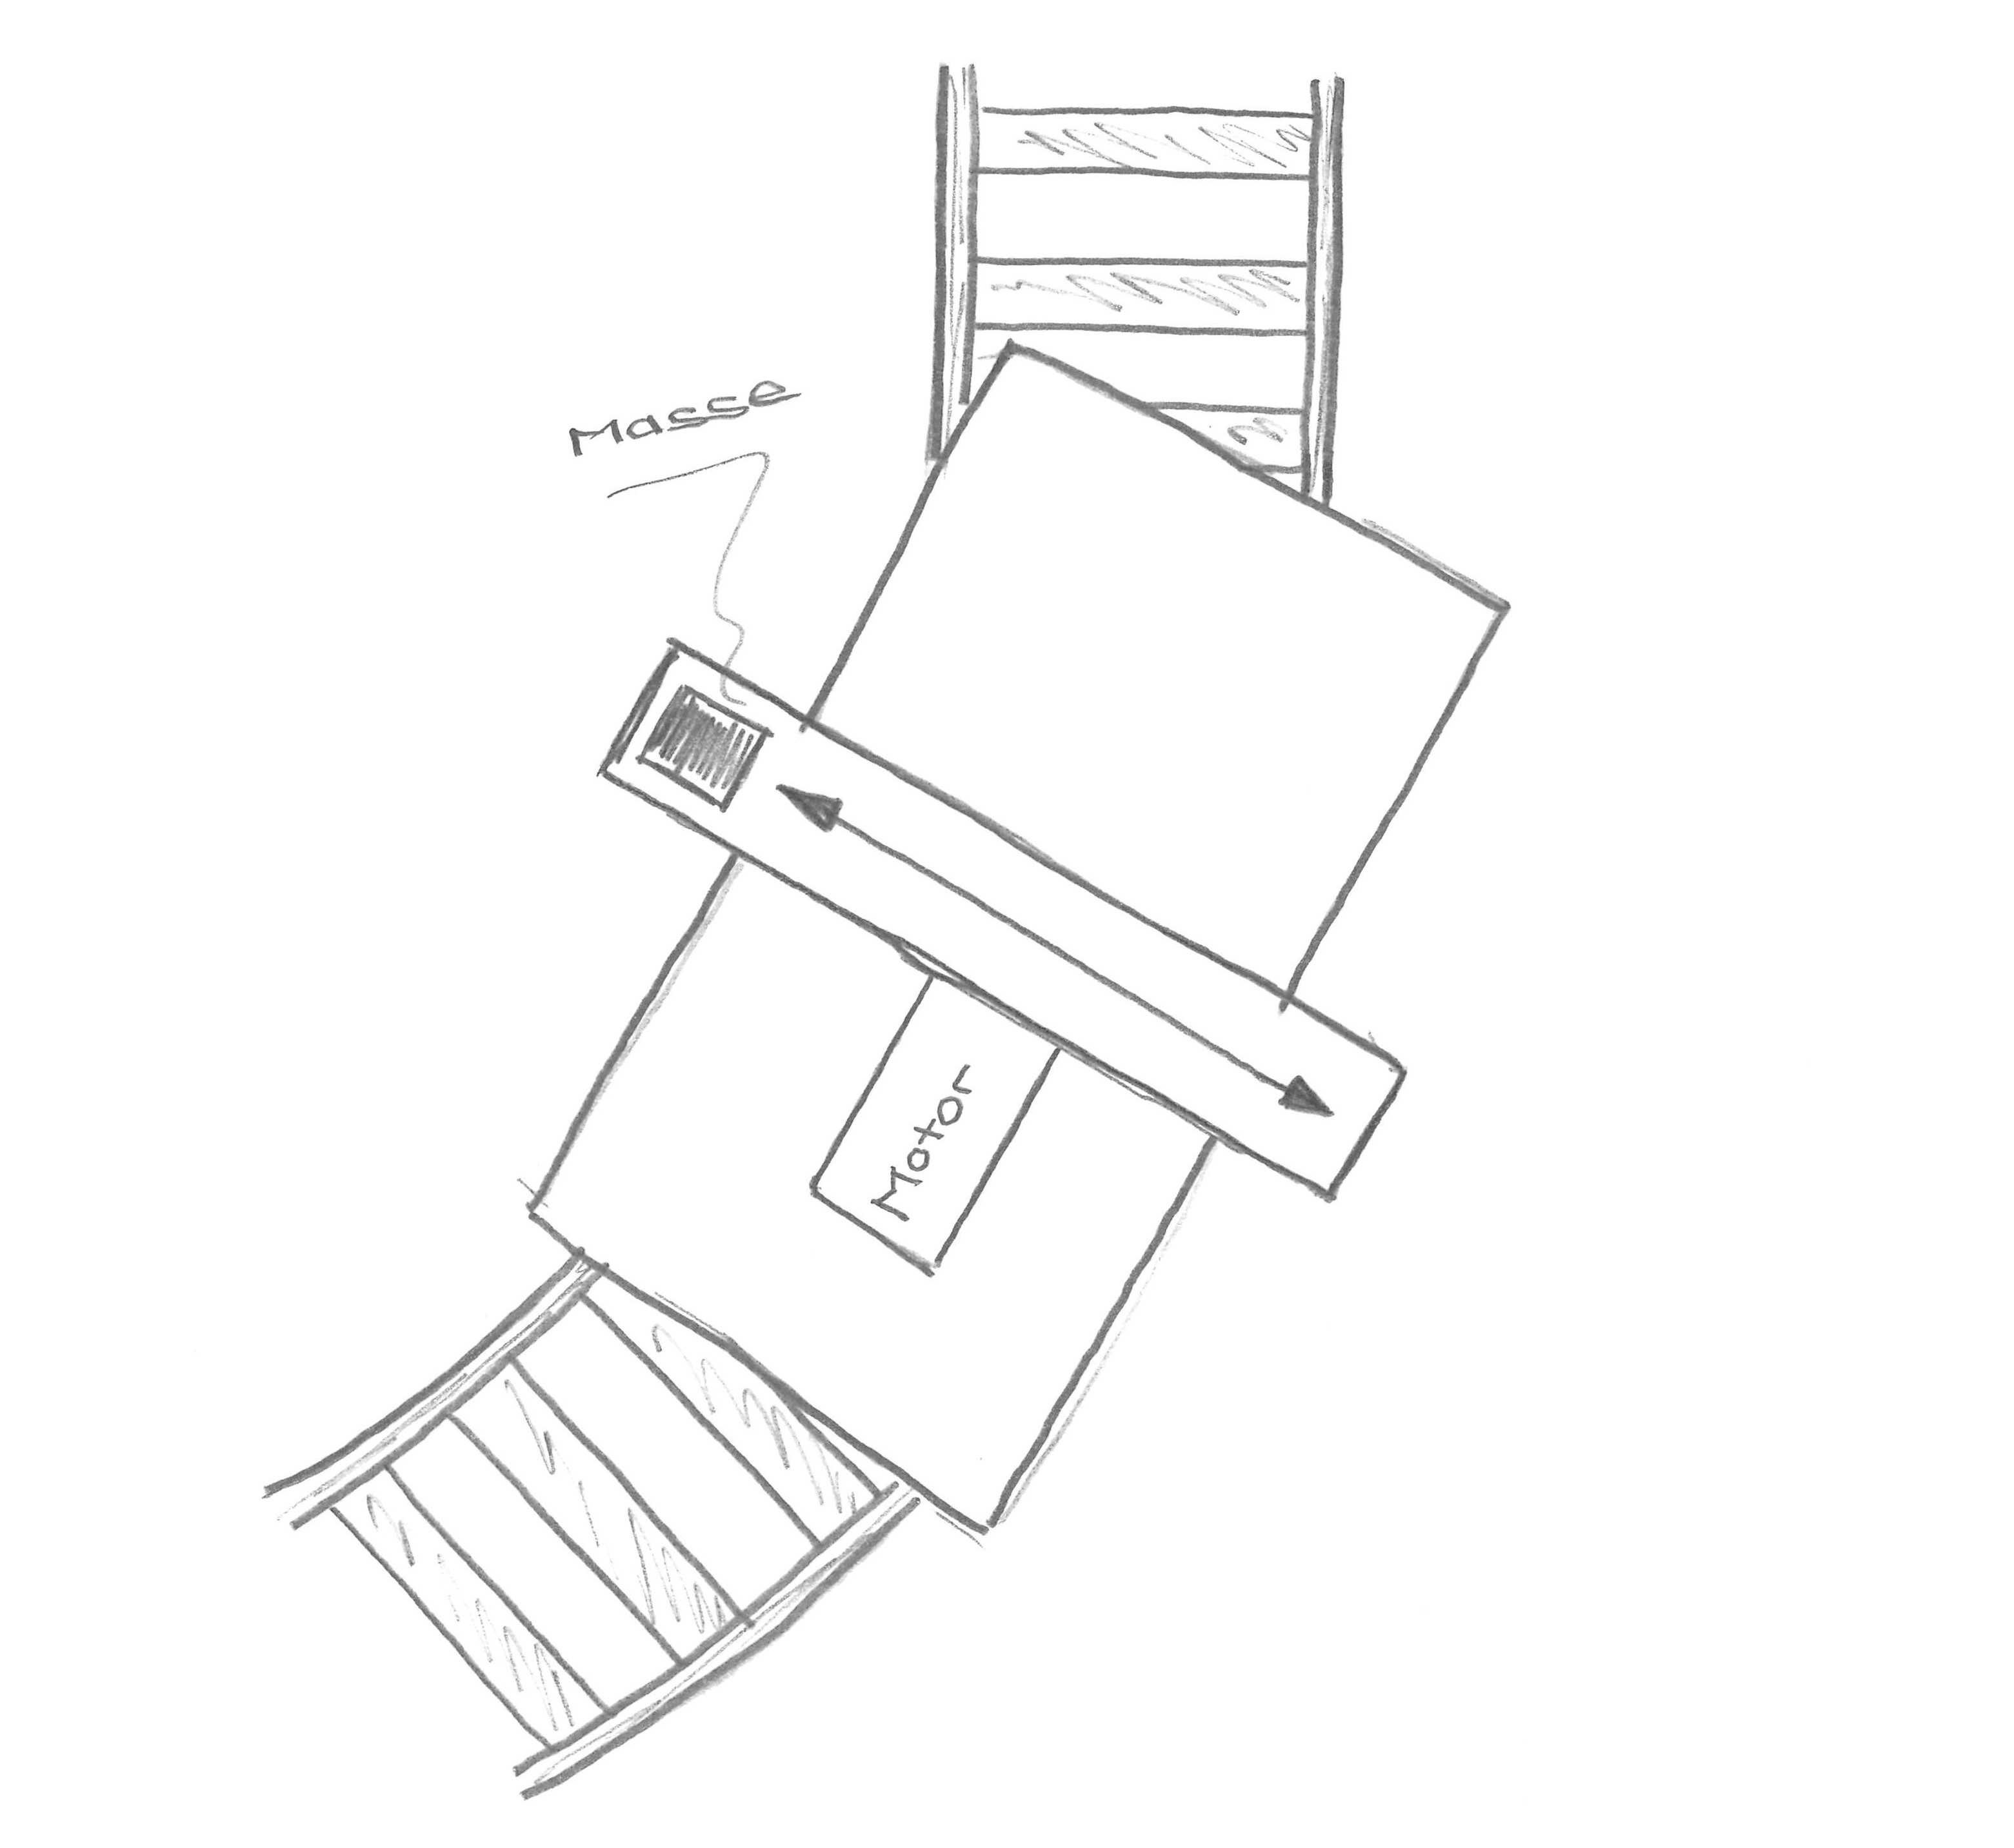
\includegraphics[width=0.8\textwidth]{Schwenker}
        \caption{Lösungskonzept Schwenker}
        \label{fig:schwenker}
    \end{figure}

    \begin{flushleft}
        \begin{table}[h]
        \begin{tabular}{ | l | p{11cm} |}
        \hline
        \textbf{Problemstellung} & Kurvenfahrt (ohne aus den Gleisen zu fallen) \\ \hline
        \textbf{Disziplin} & Maschinentechnik und Elektrotechnik \\ \hline
        \textbf{Lösungskonzept} & Schwenker \\ \hline
        \textbf{Bewertung} &  \begin{itemize}
                                \item[+] Genauigkeit der Gewichtsverlagerung
                                \item[+] Zusätzlich für das problemlose Anheben des Würfels verwendbar
                                \item[-] Preis 
                                \item[-] Mehrere Komponenten nötig 
                              \end{itemize} \\ \hline
        \end{tabular}
        \caption{Konzeptbeurteilung: Schwenker für die Kurvenfahrt}
        \label{tab:schwenker}
    \end{table}
    \end{flushleft}

    \textbf{Tiefer Schwerpunkt}\\
    Das Konzept des tiefen Schwerpunkts hat sich deshalb in der Nutzwertanalyse durchgesetzt, da kein zusätzlicher Materialaufwand und die damit verbundenen Kosten entstehen. Der Grundgedanke dieser Lösungsvariante besteht darin, das Konzept so zu gestalten, dass der Schwerpunkt so tief wie möglich gehalten werden kann. Somit ist das Moment auf den Wagen in der Kurve kleiner und es muss weniger ausglichen werden.

    \begin{flushleft}
        \begin{table}[h]
        \begin{tabular}{ | l | p{11cm} |}
        \hline
        \textbf{Problemstellung} & Kurvenfahrt (ohne aus den Gleisen zu fallen) \\ \hline
        \textbf{Disziplin} & Maschinentechnik und Elektrotechnik \\ \hline
        \textbf{Lösungskonzept} & Tiefer Schwerpunkt \\ \hline
        \textbf{Bewertung} &  \begin{itemize}
                                \item[+] Einfach
                                \item[+] Keine Kosten
                                \item[-] Ungenau 
                                \item[-] Unkontrollierbar 
                              \end{itemize} \\ \hline
        \end{tabular}
        \caption{Konzeptbeurteilung: Tiefer Schwerpunkt für die Kurvenfahrt}
        \label{tab:tieferschwerpunkt}
    \end{table}
    \end{flushleft}

    Anhand der Vor- und Nachteile der jeweiligen Lösungsvariante hat sich abgezeichnet, die Variante des Schwenkers in erster Linie weiter zu verfolgen und die Variante mit dem tiefen Schwerpunkt für eine zweite alternative Variante zu wählen.
    
    \textbf{Bremsen}\\
    Ein Ziel des Schienenfahrzeugs ist es, möglichst schnell einen variablen Kurs autonom abzufahren. Damit man auf den geraden Strecken mit der Höchstgeschwindigkeit fahren kann und die Kurven kriegen will, braucht es eine kontrollierte Geschwindigkeitsreduktion. Nach der Nutzwertanalyse (siehe Abbildung \ref{fig:bremsen}) haben sich die Bremsung mittels Motor und Steuerung sowie eine mechanische Bremse direkt auf die Räder durchgesetzt.

    \begin{figure}[H] %Nutzwertanalyse Bremsen
        \centering
        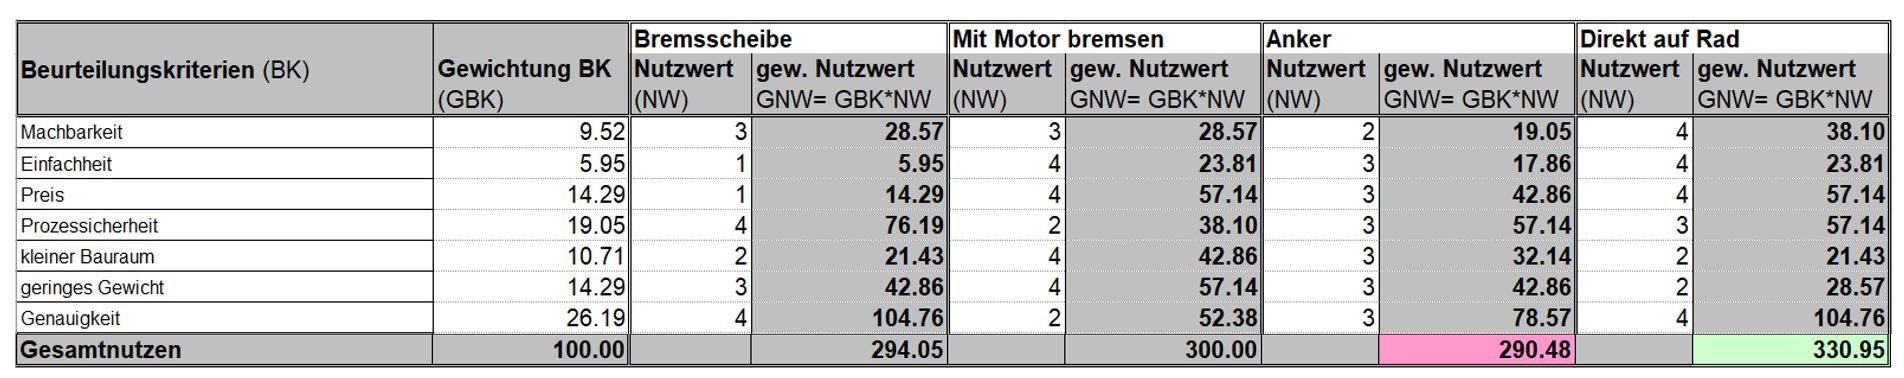
\includegraphics[width=1\textwidth]{Bremsen}
        \caption{Nutzwertanalyse Bremsen}
        \label{fig:bremsen}
    \end{figure}

    \textbf{Motorbremse}\\
    Sobald die Steuerung eine Kurve erkennt, kann sie den Motor mit der Stromregelung bremsen. Das ist eine mechanisch einfache Variante und kann rein auf der Steuerung aufbauen. (siehe Tabelle \ref{tab:motorbremse})

    \begin{flushleft}
        \begin{table}[h]
        \begin{tabular}{ | l | p{11cm} |}
        \hline
        \textbf{Problemstellung} & Bremsen \\ \hline
        \textbf{Disziplin} & Maschinentechnik \\ \hline
        \textbf{Lösungskonzept} & Bremsklotz direkt auf Rad \\ \hline
        \textbf{Bewertung} &  \begin{itemize}
                                \item[+] Einfach
                                \item[+] Geringe Kosten
                                \item[+] Stetige Kontrolle über Bremswirkung 
                                \item[-] Mehraufwand für die Elektrotechnik 
                              \end{itemize} \\ \hline
        \end{tabular}
        \caption{Konzeptbeurteilung: Bremsen mit Motor}
        \label{tab:motorbremse}
    \end{table}
    \end{flushleft}

    \textbf{Radbremse}\\
    Wie es der Titel schon sagt, wird die Bremswirkung (siehe Abbildung \ref{fig:tab:radbremse} mittels Reibung eines Bremsklotzes auf dem Rad erzeugt (siehe Tabelle \ref{tab:radbremse}).

    \begin{figure}[H] %Skizze Radbremse
        \centering
        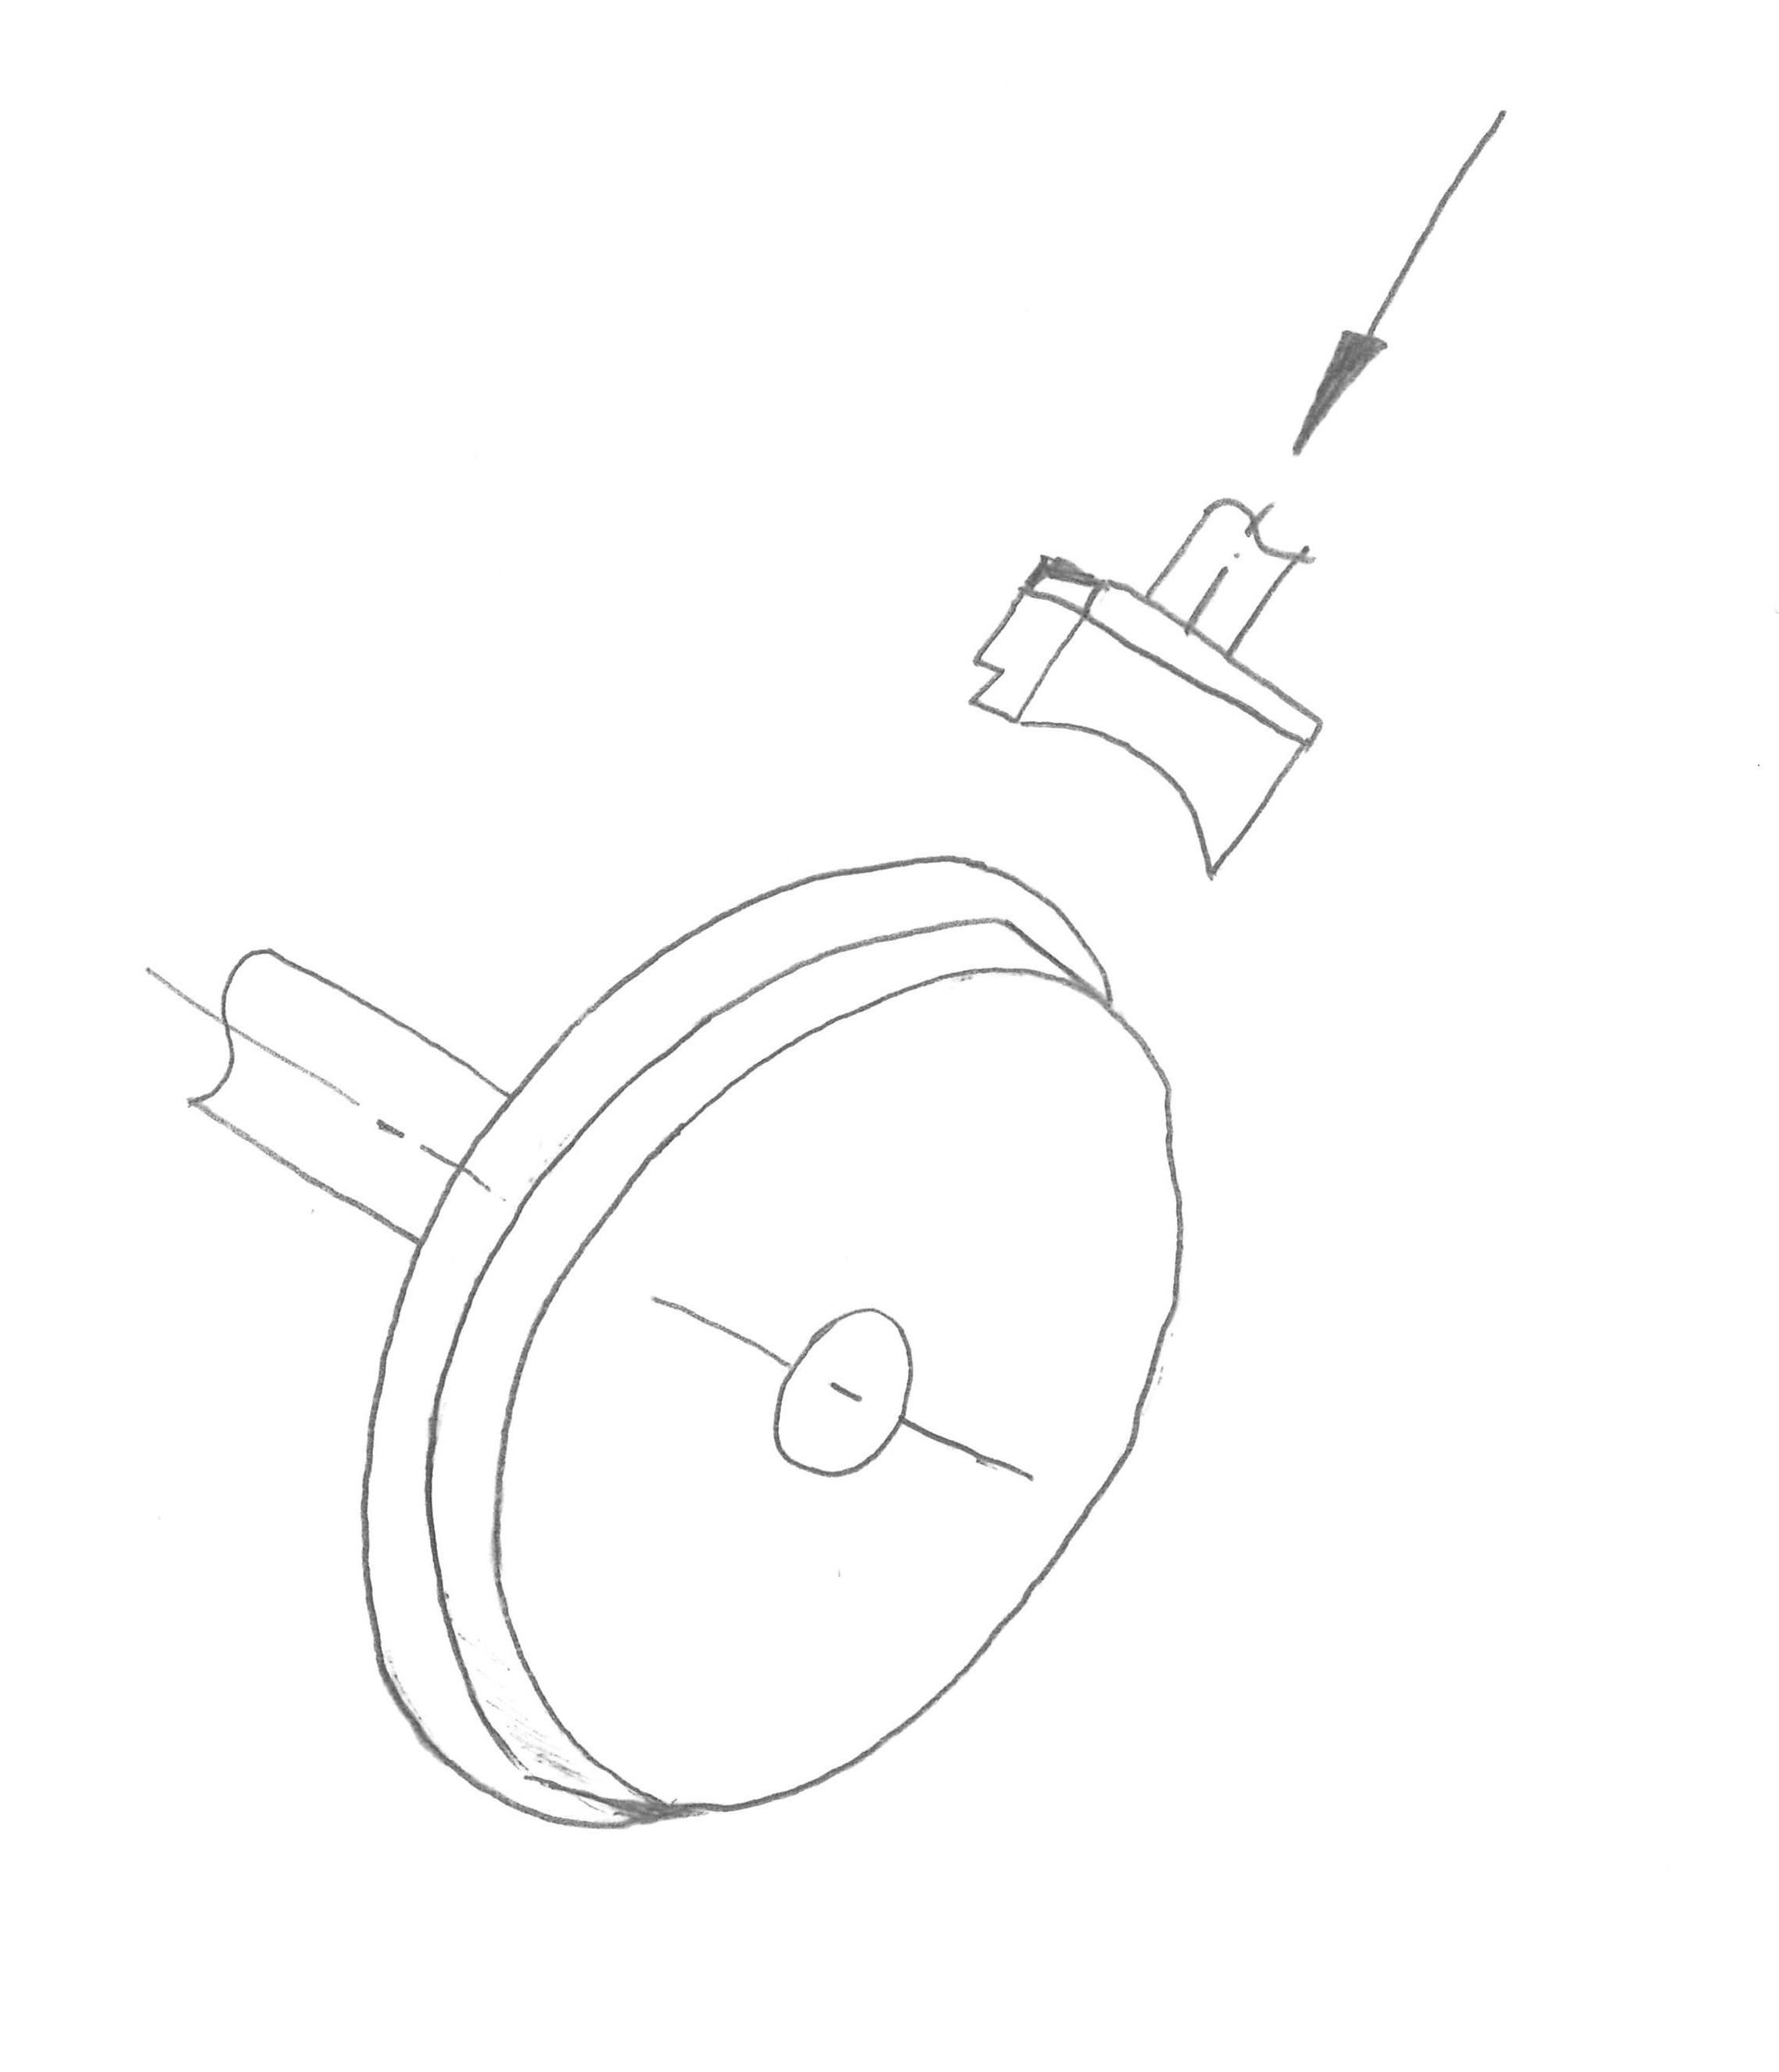
\includegraphics[width=0.5\textwidth]{Radbremse}
        \caption{Lösungskonzept Radbremse}
        \label{fig:radbremse}
    \end{figure}

\begin{flushleft}
    \begin{table}[h]
    \begin{tabular}{ | l | p{11cm} |}
    \hline
    \textbf{Problemstellung} & Bremsen \\ \hline
    \textbf{Disziplin} & Elektrotechnik \\ \hline
    \textbf{Lösungskonzept} & Bremsklotz direkt auf Rad \\ \hline
    \textbf{Komponenten} & Aktor zur Auslösung und Bremsklotz \\ \hline
    \textbf{Bewertung} &  \begin{itemize}
                            \item[+] Effiziente Energievernichtung
                            \item[+] Zuverlässigkeit
                            \item[-] Komplexität 
                            \item[-] Hohe Kosten
                          \end{itemize} \\ \hline
    \end{tabular}
    \caption{Konzeptbeurteilung: Bremsen über Rad}
    \label{tab:radbremse}
\end{table}
\end{flushleft}

  \textbf{Dämpfung}
  Die Teilfunktion Dämpfen soll das Fahrwerk des Zuges vor abrupten Schlägen und Erschütterungen schützen, womit eine kontrollierte Fahrt des Zuges ermöglicht werden soll. Anhand der Nutzwertanalyse (siehe Abbildung \ref{fig:daempfung}) haben sich die beiden Lösungskonzepte «Stossdämpfer» und «keine Dämpfung» als die Besten Lösungen dieses Problems herausgestellt.

  \begin{figure}[H] %Nutzwertanalyse Dämpfung
    \centering
    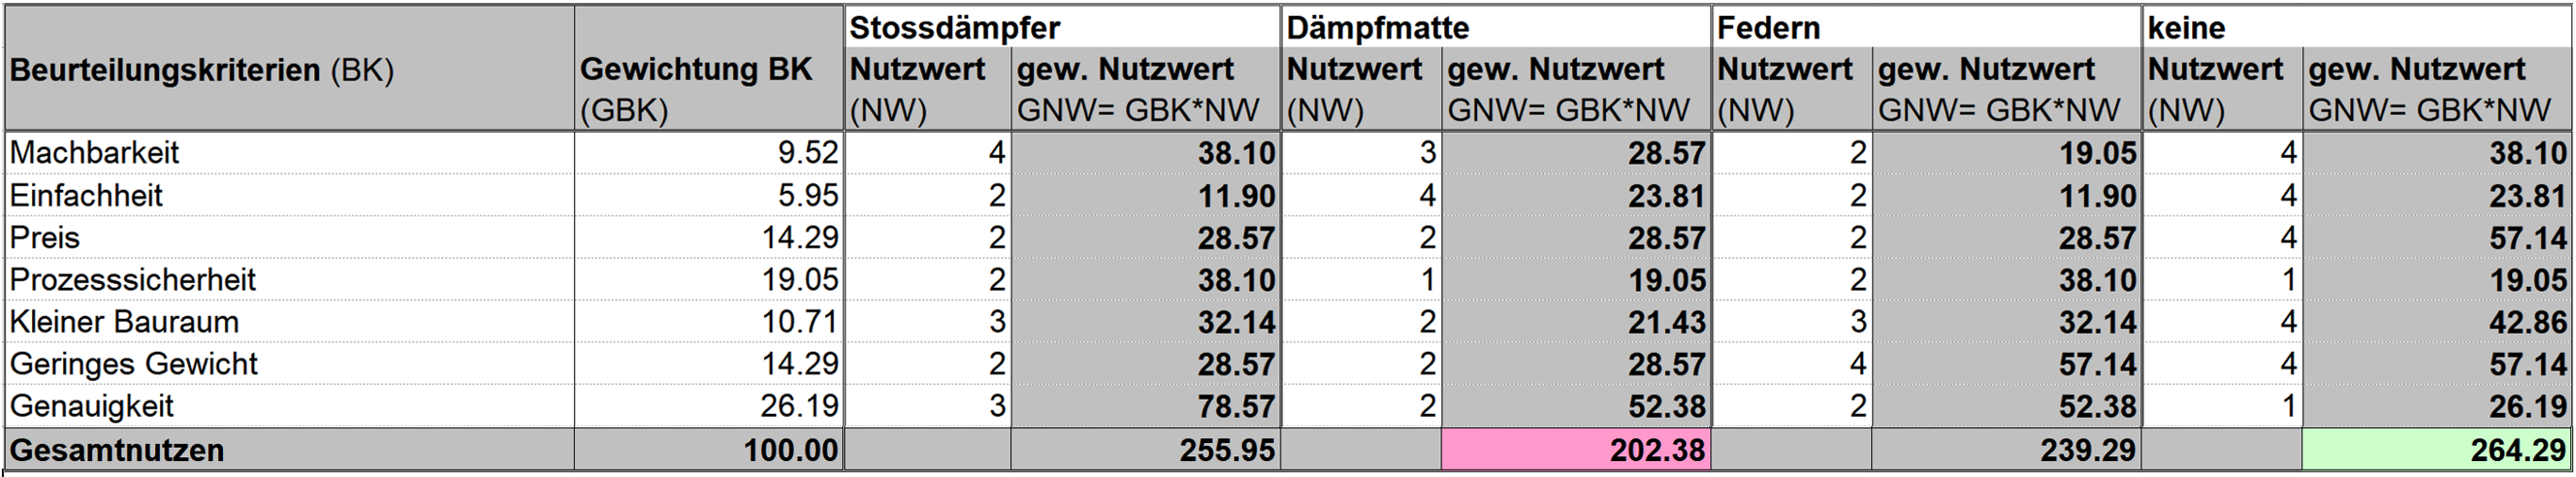
\includegraphics[width=1\textwidth]{Daempfung}
    \caption{Nutzwertanalyse Dämpfung}
    \label{fig:daempfung}
\end{figure}

  \textbf{Stossdämpfer}\\
  Der Stossdämpfer (siehe Abbildung \ref{fig:stossdaempfer}) ist ein handelsübliches Einkaufsteil, dass durch seine Einfachheit und den geringen Preis für diese Problemstellung optimal ist. Er sollte einstellbar sein. Die Vor- und Nachteile dieses Konzeptes sind in der Tabelle \ref{tab:stossdaempfer}) aufgelistet.

  \begin{figure}[H] %Bild Stossdaempfer
    \centering
    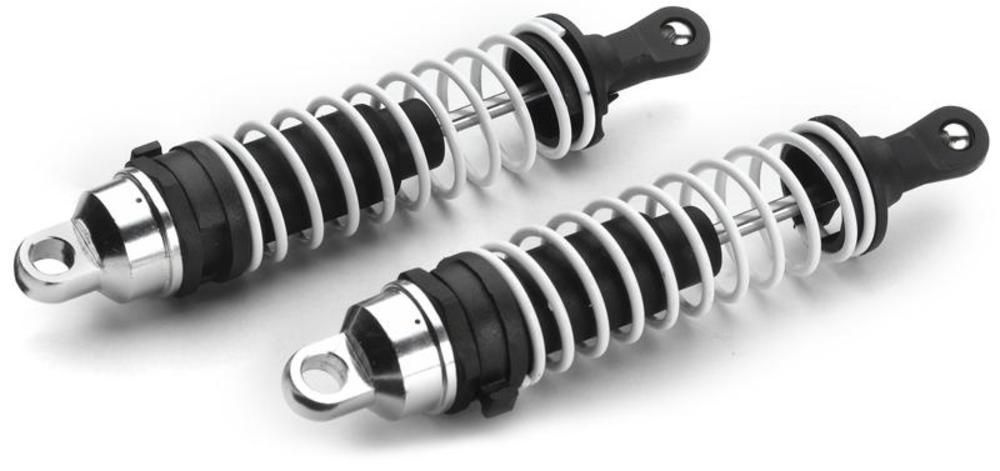
\includegraphics[width=0.7\textwidth]{Stossdaempfer}
    \caption{Lösungskonzept Stossdämpfer}
    \label{fig:stossdaempfer}
  \end{figure}

  \begin{flushleft}
    \begin{table}[h]
    \begin{tabular}{ | l | p{11cm} |}
    \hline
    \textbf{Problemstellung} & Dämpfung (für eine laufruhige Fahrt) \\ \hline
    \textbf{Disziplin} & Maschinentechnik \\ \hline
    \textbf{Lösungskonzept} & Stossdämpfer \\ \hline
    \textbf{Bewertung} &  \begin{itemize}
                            \item[+] Einfach
                            \item[+] Kosten
                            \item[-] Machbarkeit (aufwändig)
                          \end{itemize} \\ \hline
    \end{tabular}
    \caption{Konzeptbeurteilung: Dämpfen mit Stossdämpfer}
    \label{tab:stossdaempfer}
\end{table}
\end{flushleft}

\textbf{Keine Dämpfung}\\
Neben den vielen Möglichkeiten den Zug vor Schlägen und Unebenheiten zu schützen besteht ebenfalls die Möglichkeit komplett auf eine Dämpfung zu verzichten, da auf der Fahrbahn mit sehr wenig Störungen zu rechnen ist. Es besteht jedoch die Möglichkeit des Einsatzes von Dämpfungen bei vereinzelten Komponenten wie der Kamera, falls dies erforderlich ist (siehe Tabelle \ref{tab:keinedaempfung}).

\begin{flushleft}
    \begin{table}[h]
    \begin{tabular}{ | l | p{11cm} |}
    \hline
    \textbf{Problemstellung} & Dämpfung (für eine laufruhige Fahrt) \\ \hline
    \textbf{Disziplin} & Maschinentechnik \\ \hline
    \textbf{Lösungskonzept} & Keine Dämpfung \\ \hline
    \textbf{Bewertung} &  \begin{itemize}
                            \item[+] Keine Kosten
                            \item[-] Erschütterungen bei der Fahrt möglich
                          \end{itemize} \\ \hline
    \end{tabular}
    \caption{Konzeptbeurteilung: Dämpfen mit Stossdämpfer}
    \label{tab:keinedaempfung}
\end{table}
\end{flushleft}

Anhand der Bewertungskriterien und der genauen Betrachtung der Sachlage stellt sich heraus, dass es für das Endprodukt nicht von grosser Bedeutung ist, ob eine Dämpfung vorhanden ist oder nicht. Der Aufwand gegenüber dem Nutzen wird als wesentlich grösser erachtet. Deshalb wird für die favorisierte Lösung keine Dämpfung zum Einsatz kommen.

\subsubsection{Würfeltransport}

\textbf{Greifen}
 Eine Teilfunktion des Hochgeschwindigkeitsschienenfahrzeugs beinhaltet das Greifen eines Würfels. Dieser weist eine Kantenlänge von jeweils 50 cm auf und ist mit einem Hacken ausgestattet der auf der oberen Seite platziert ist und die Öffnung entgegen der Fahrtrichtung zeigt. Der Abstand des Würfels zur Gleismitte ist gegeben, nur die Position entlang der Gleise ist unbekannt. Ziel des Vorrichtung ist es nun, diesen Würfel zu Greifen und anschliessen auf dem Schienenfahrzeug zu platzieren. In folgendem Abschnitt werden die zwei besten Lösungen anhan der Nutzwertanalyse für diese Problemstellung vorgestellt.

 \begin{figure}[H] %Nutzwertanalyse Greifen
    \centering
    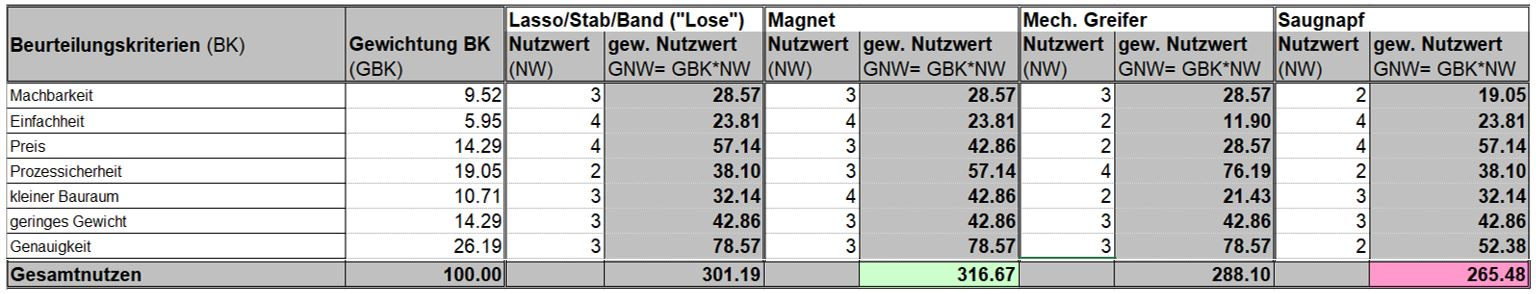
\includegraphics[width=1\textwidth]{Greifen}
    \caption{Nutzwertanalyse Greifen}
    \label{fig:greifen}
\end{figure}

     \textbf{Stab}\\
 Der Stab in Abbildung \ref{fig:stab} wurde gemäss Nutzwertanalyse (siehe Tabelle \ref{tab:stab}) als zweit beste Lösungsvariante ausgegeben, wird aber trotzdem favorisiert, weil die Einfachheit der Vorrichtung und die definierte Position des Würfels überzeugen. Ergänzend zum Stab soll ein beweglicher Haken einhängen können.

 \begin{figure}[H] %Skizze Stab
    \centering
    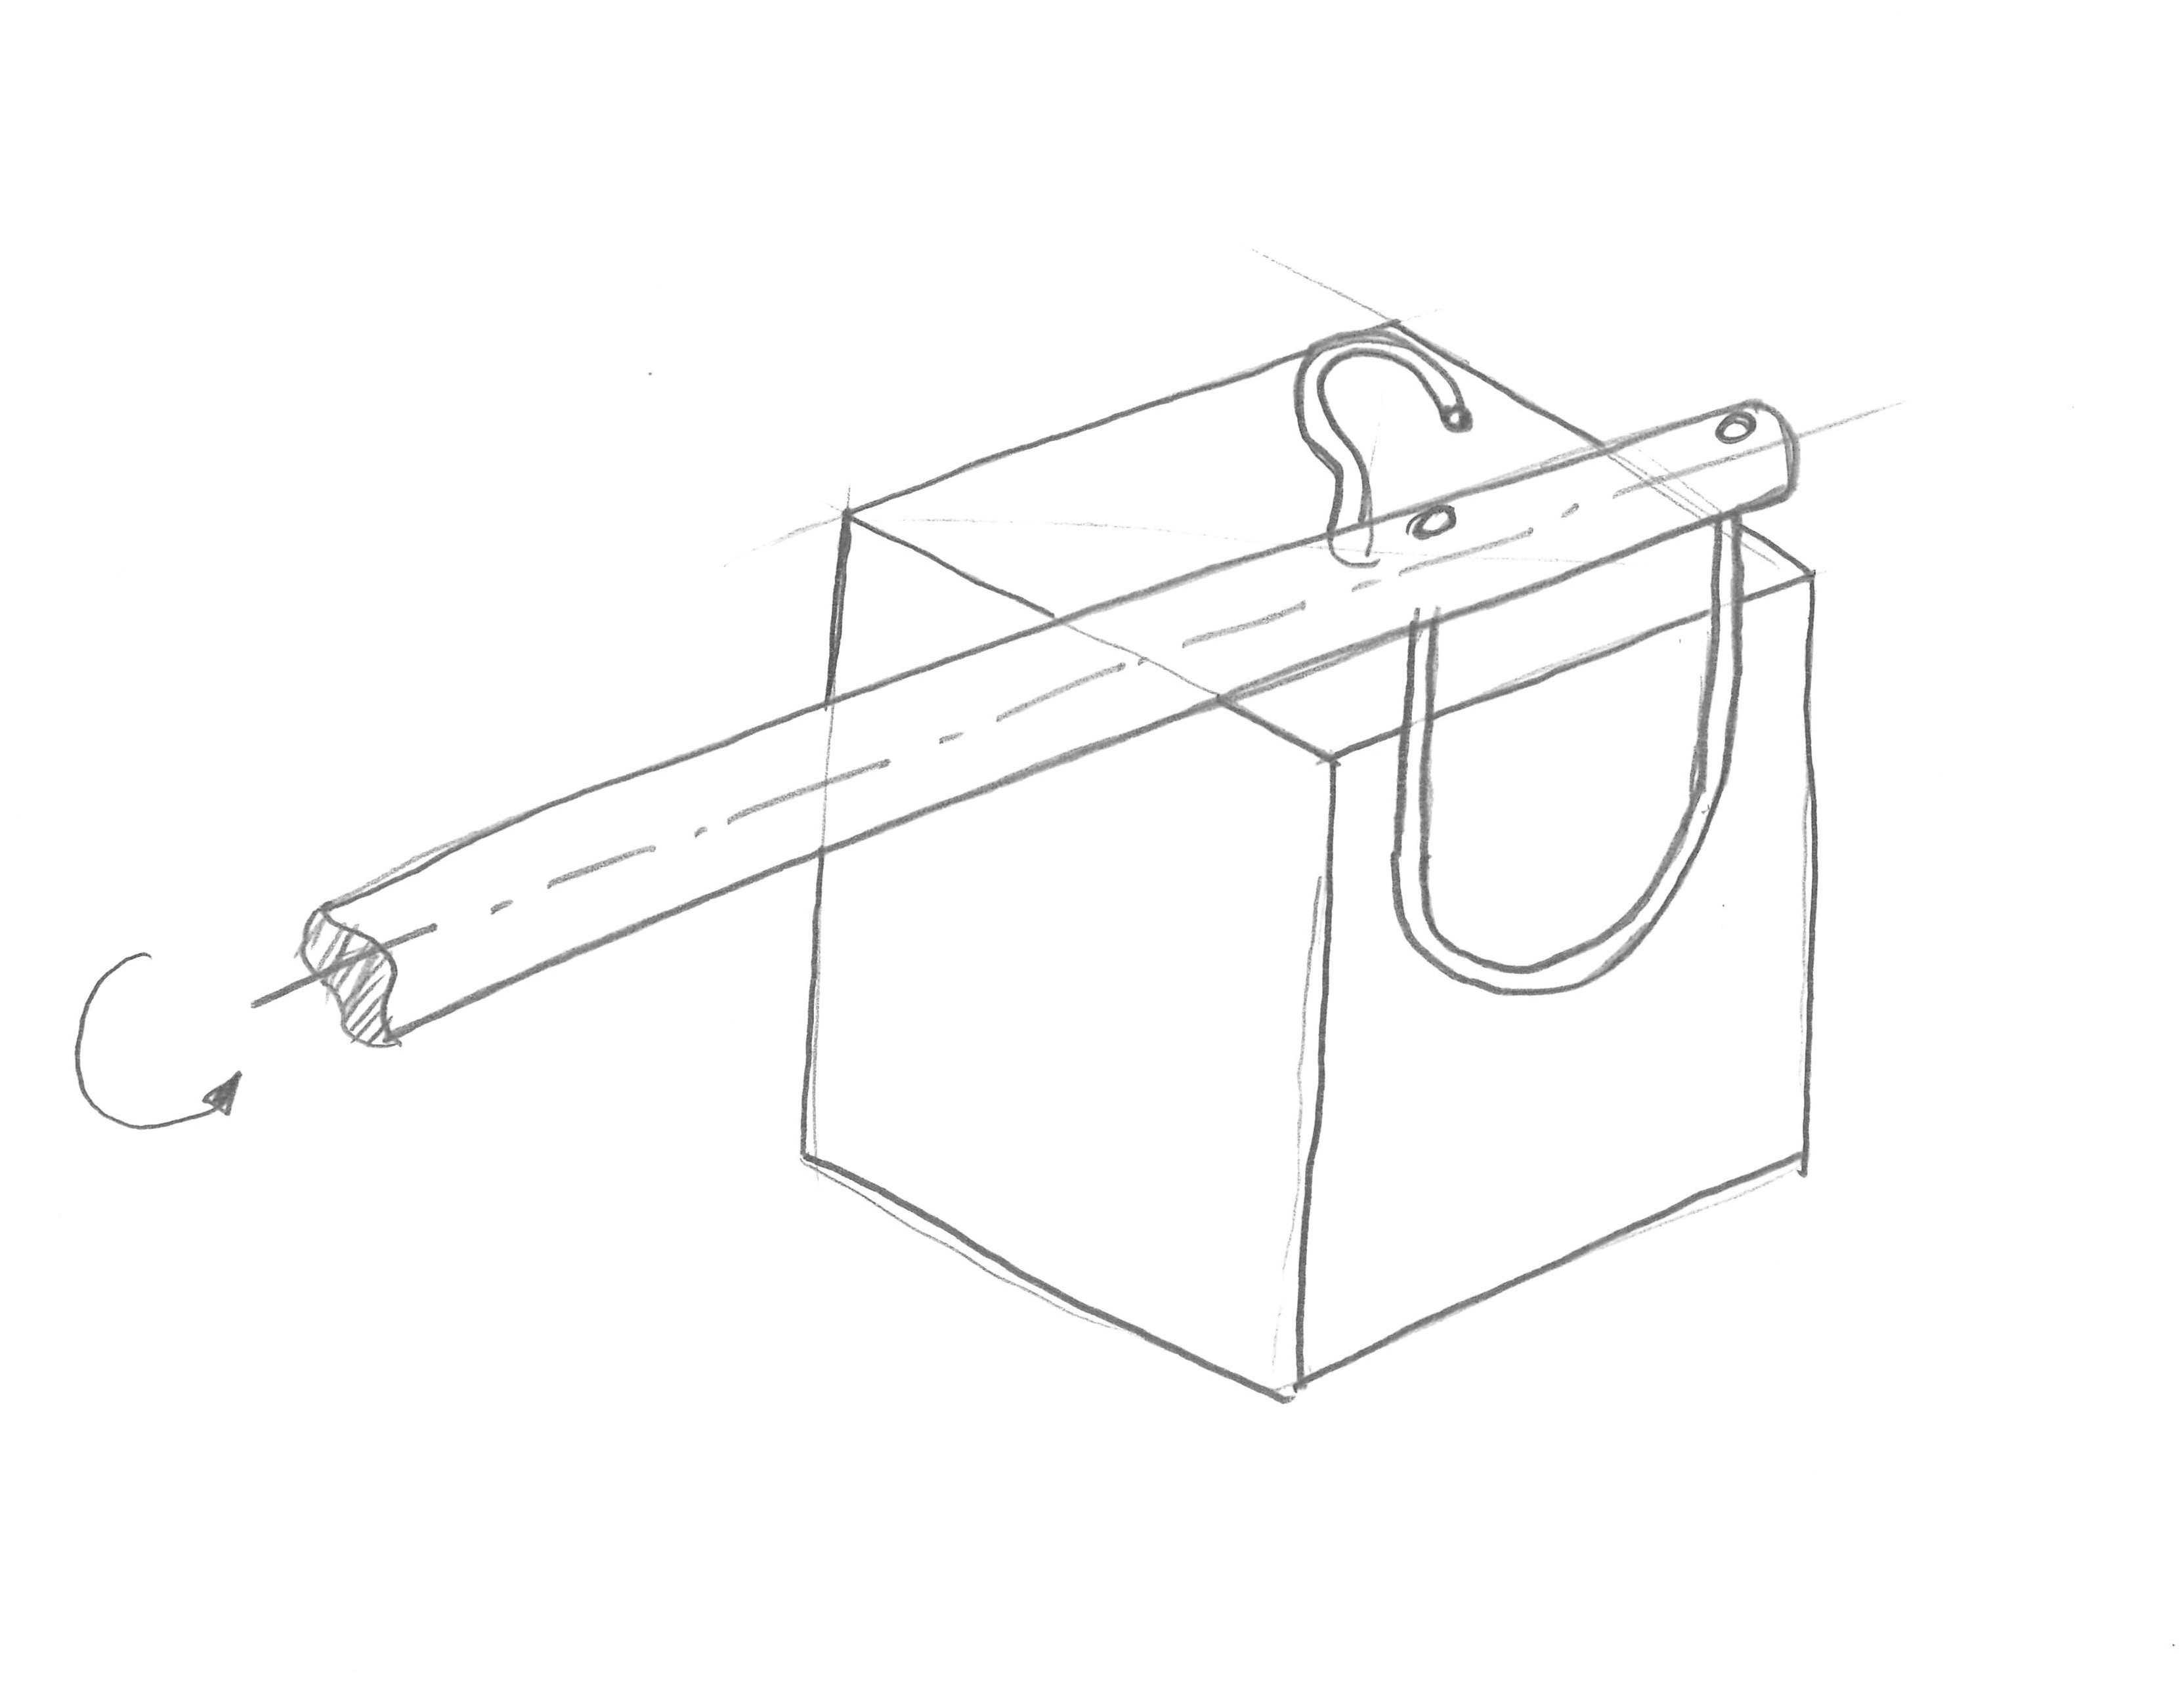
\includegraphics[width=0.8\textwidth]{Stab}
    \caption{Lösungskonzept Stab}
    \label{fig:stab}
\end{figure}

\begin{flushleft}
    \begin{table}[h]
    \begin{tabular}{ | l | p{11cm} |}
    \hline
    \textbf{Problemstellung} & Würfeltransport: Greifen \\ \hline
    \textbf{Disziplin} & Maschinentechnik \\ \hline
    \textbf{Lösungskonzept} &  Stab \\ \hline
    \textbf{Komponente} & Stab und Haken \\ \hline
    \textbf{Bewertung} &  \begin{itemize}
                            \item[+] Positionierung
                            \item[+] Einfachheit
                            \item[+] Erfolgsgarantie 
                            \item[-] Auslenkung
                          \end{itemize} \\ \hline
    \end{tabular}
    \caption{Konzeptbeurteilung: Würfeltransport mittels Stab}
    \label{tab:stab}
\end{table}
\end{flushleft}

\textbf{Magnet}\\
 Der Haken des Würfels wird auf magnetischem Material sein und so sollte definitiv eine Lösungsvariante mit einem Magneten in Betracht gezogen werden. Diese Variante ist in der Bewertung vorne mit dabei, doch auf Grund der unberechenbaren Kräfte und Auslenkungen des Würfels hat man sich gegen einen Magneten entschieden. Falls die erste Option nicht die gewünschten Ergebnisse bringt, wird der Magnet zum Plan B und der Vorgang muss mit einigen Tests und Szenarien geprüft werden.

 \begin{flushleft}
    \begin{table}[h]
    \begin{tabular}{ | l | p{11cm} |}
    \hline
    \textbf{Problemstellung} & Würfeltransport: Greifen \\ \hline
    \textbf{Disziplin} & Maschinentechnik \\ \hline
    \textbf{Lösungskonzept} &  Magnet \\ \hline
    \textbf{Komponente} & Magnet und Führung \\ \hline
    \textbf{Bewertung} &  \begin{itemize}
                            \item[+] Kompakte Bauweise
                            \item[+] Einfachheit
                            \item[-] unberechenbar 
                            \item[-] keine Wiederholgenauigkeit
                          \end{itemize} \\ \hline
    \end{tabular}
    \caption{Konzeptbeurteilung: Würfeltransport mittels Magnet}
    \label{tab:konzept_wurfeltrransport_magnet}
\end{table}
\end{flushleft}
\textbf{Verschieben und Platzieren}
Nachdem der Würfel im Startbereich der Strecke korrekt gegriffen wurde, wird er in einem nächsten Schritt verschoben und auf dem Zug platziert. Dazu haben sich die beiden Lösungsvorschläge «Um- und Einschwenker» und «Rampe mit Seilzug» in der Nutzwertanalyse durchgesetzt. In folgendem Abschnitt werden die zwei besten Lösungen anhan der Nutzwertanalyse (siehe Abbildung \ref{fig:verschieben_platzieren}) für diese Problemstellung vorgestellt.

\begin{figure}[H] %Nutzwertanalyse Verschieben
    \centering
    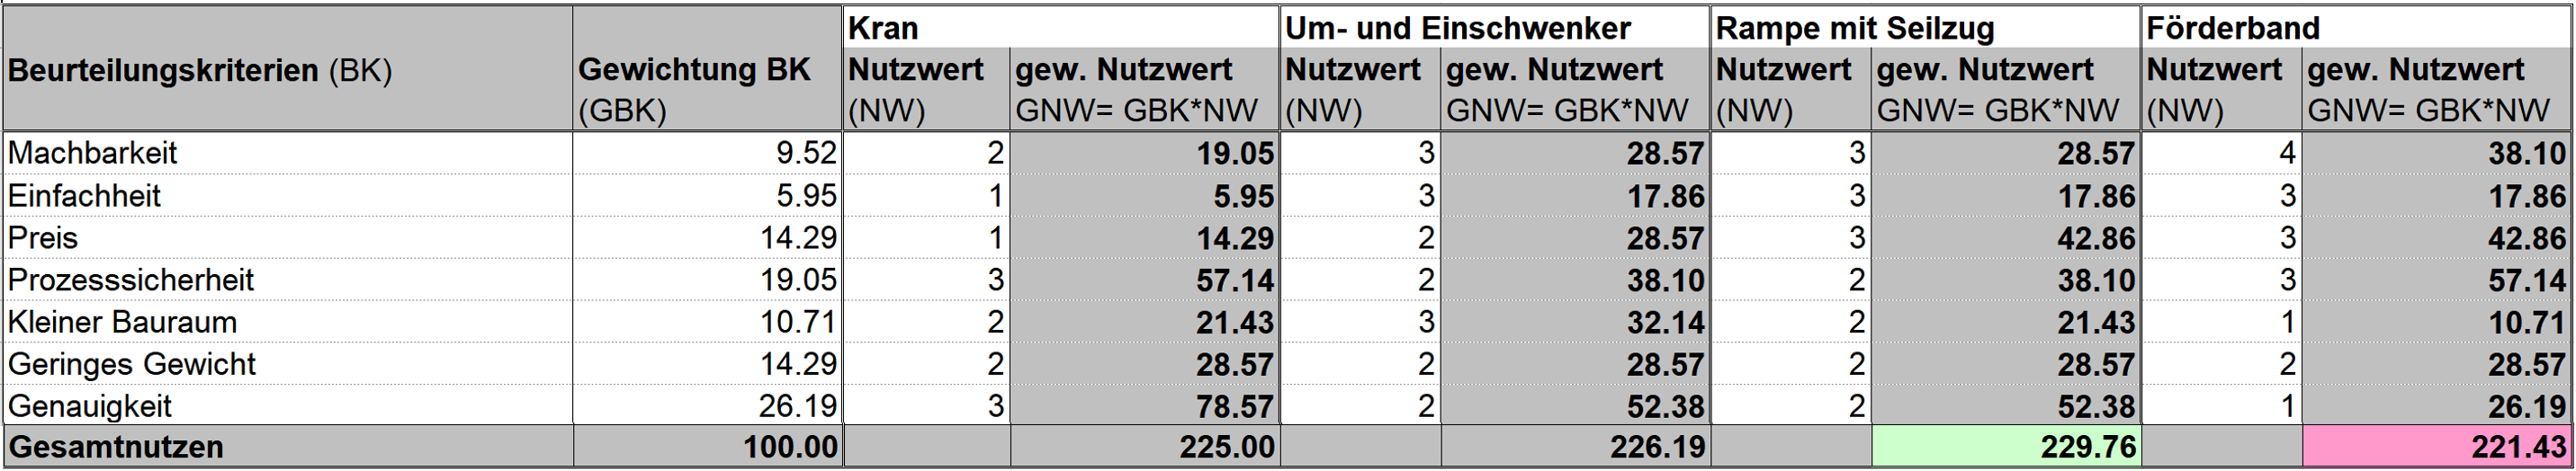
\includegraphics[width=1\textwidth]{Verschieben_platzieren}
    \caption{Nutzwertanalyse Verschieben und Platzieren}
    \label{fig:verschieben_platzieren}
\end{figure}
\pagebreak
\textbf{Um- und Einschwenker}\\
Der Um- und Einschwenker in Abbildung \ref{fig:umschenker} ist ein Konzept, in welchem versucht wird die Bewegung des Verschiebens nur durch eine Achse zu realisieren. Somit bleibt das System einfach und übersichtlich. Es ist aber noch offen, um welche Achse sich der Schwenker drehen soll - entweder schwenkt er seitwärts zum Zug ein (Einschwenker) oder auf den Zug herauf (Umschwenker).

\begin{figure}[H] %Skizze Um- und Einschwenker
    \centering
    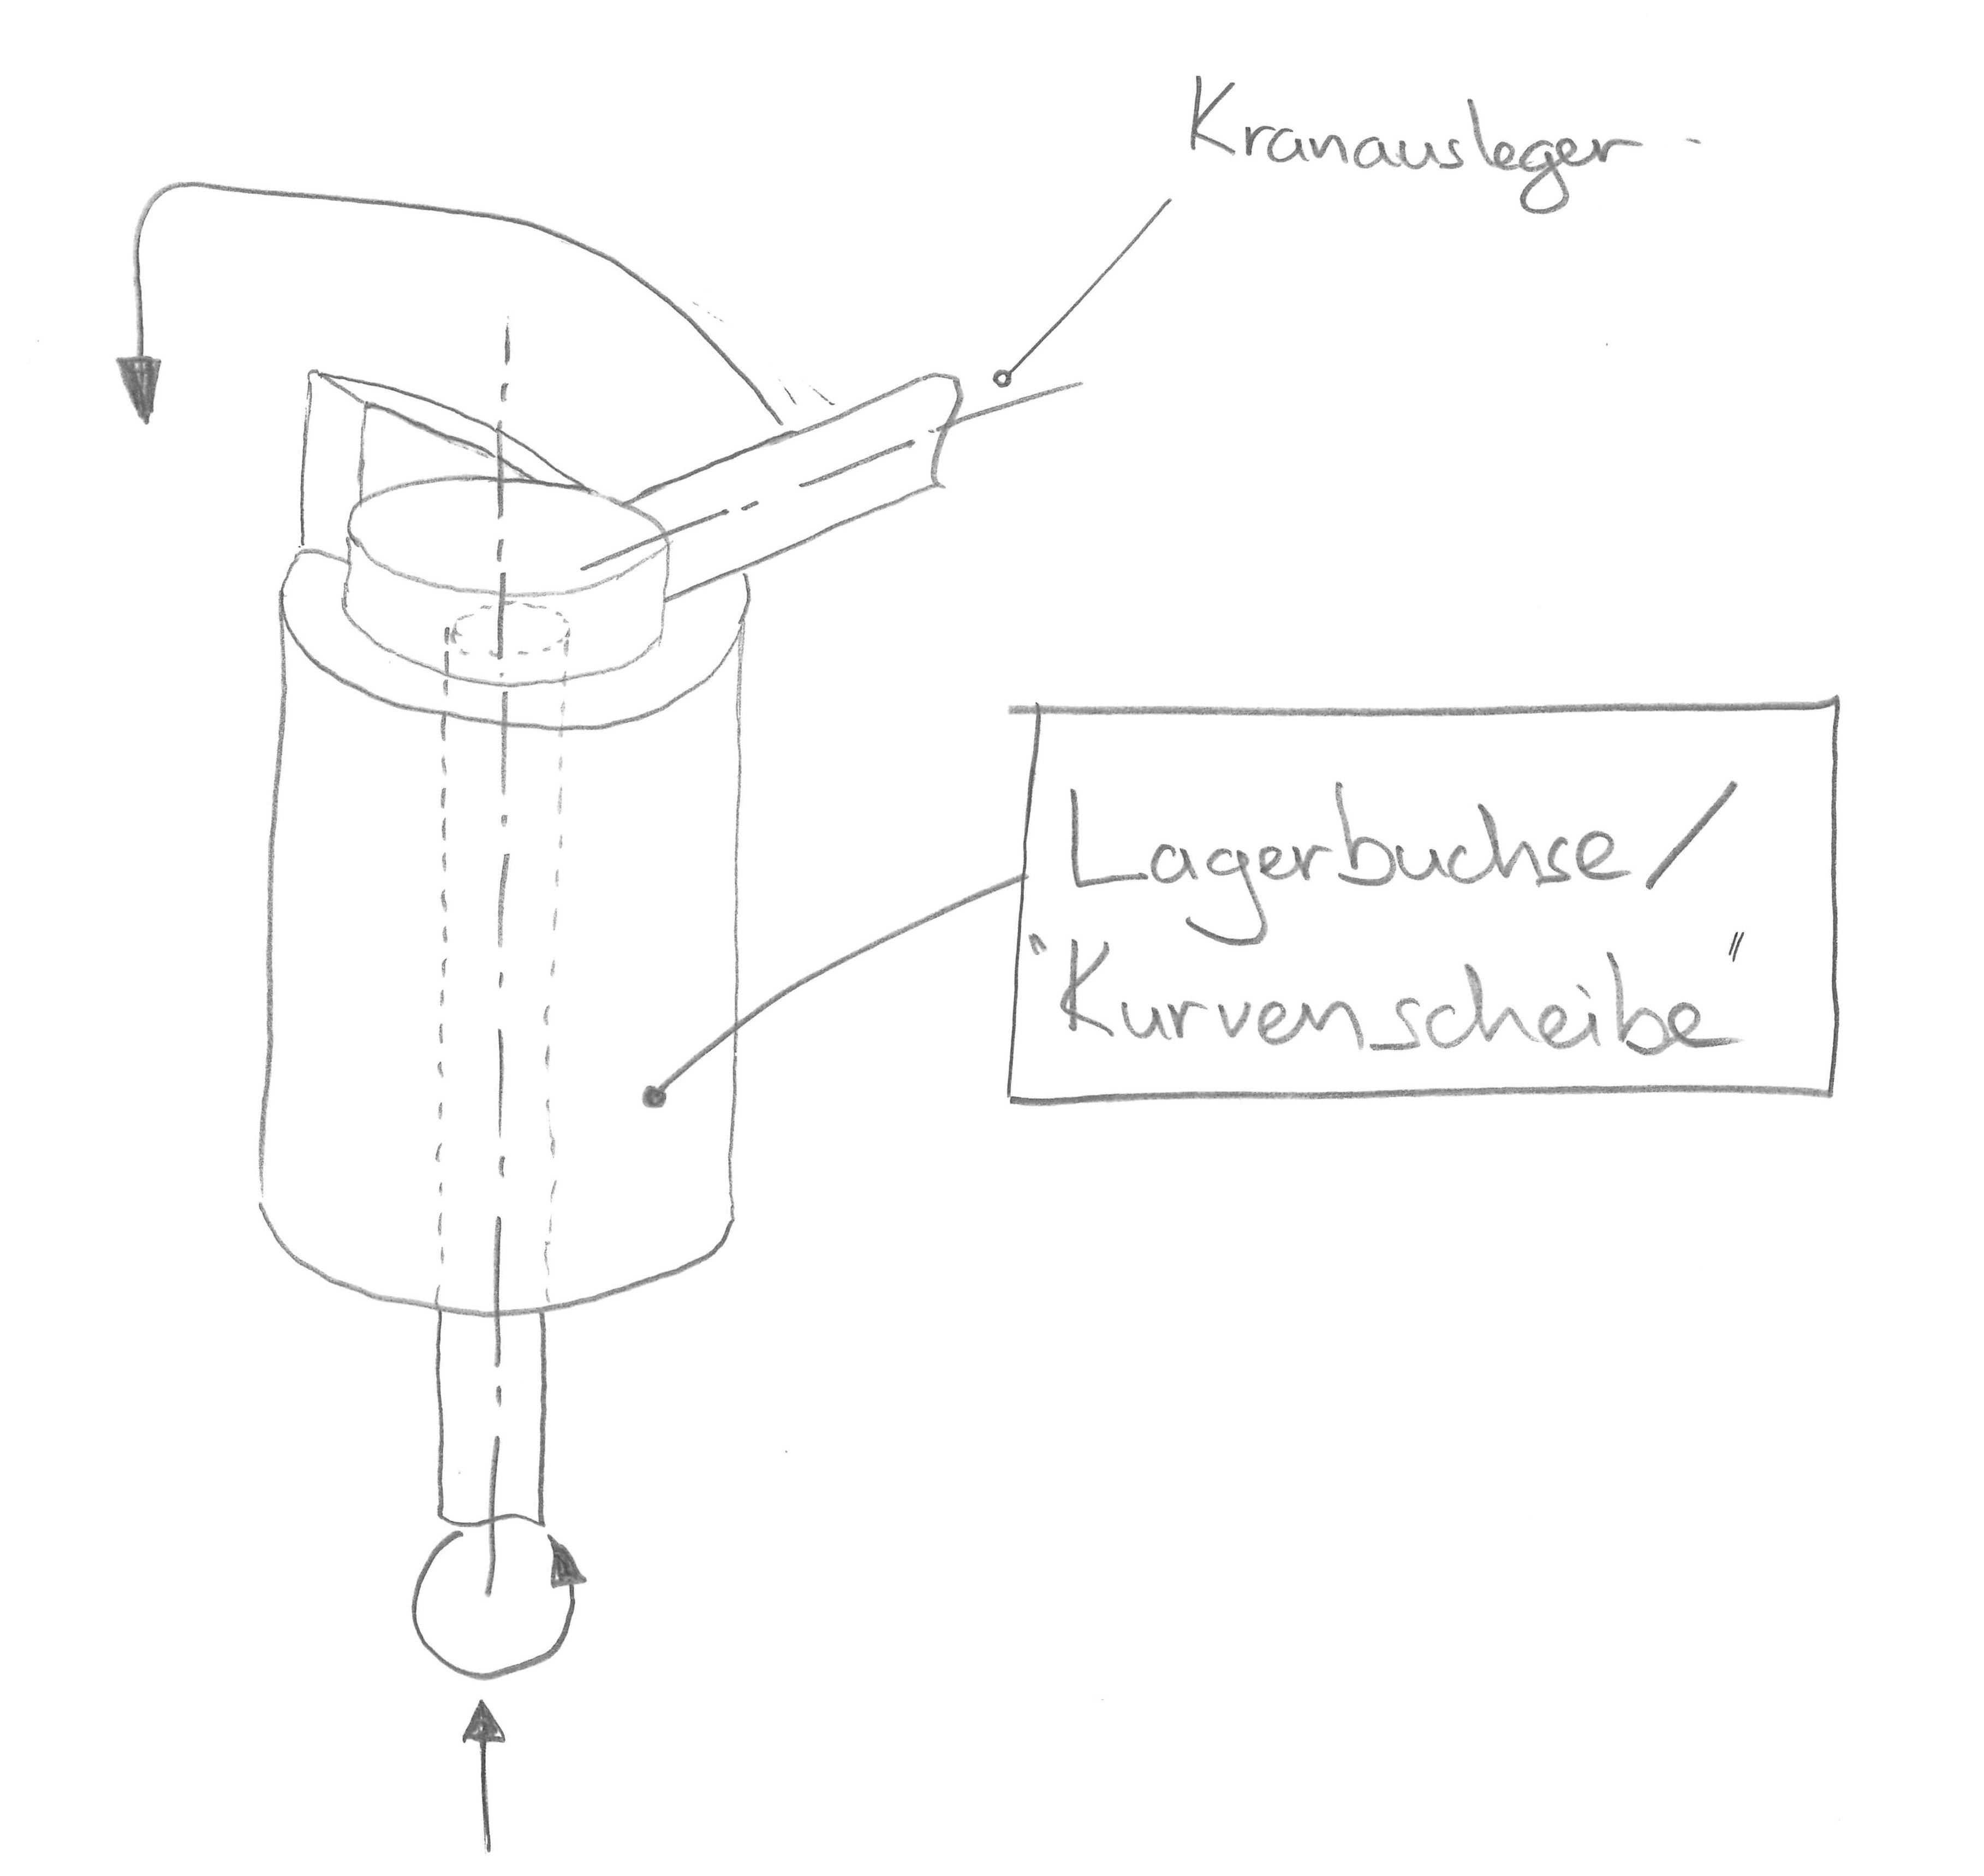
\includegraphics[width=0.8\textwidth]{Umschenker}
    \caption{Lösungskonzept Um- und Einschwenker}
    \label{fig:umschenker}
\end{figure}

\begin{flushleft}
    \begin{table}[h]
    \begin{tabular}{ | l | p{11cm} |}
    \hline
    \textbf{Problemstellung} & Würfeltransport: Verschieben \\ \hline
    \textbf{Disziplin} & Maschinentechnik \\ \hline
    \textbf{Lösungskonzept} &  Um- und Einschwenker \\ \hline
    \textbf{Bewertung} &  \begin{itemize}
                            \item[+] Bewegung erfolgt nur auf einer Achse
                            \item[+] Einfachheit
                            \item[+] tiefer Schwerpunkt
                            \item[-] Grosser Bauraum
                          \end{itemize} \\ \hline
    \end{tabular}
    \caption{Konzeptbeurteilung: Würfeltransport mittels Um- und Einschwenker}
    \label{tab:konzept_wurfeltrransport_umschwenker}
\end{table}
\end{flushleft}

\textbf{Rampe}
Die Lösungsvariante der Rampe (siehe Abbidlugn \ref{fig:rampe}) mit einem Seilzug bietet ebenfalls die Möglichkeit die Bewegung der Verschiebung des Würfels um eine Achse, die Seiltrommel, auszuführen. Nachdem der Würfel gepackt wurde, wird er über einen Seilzug der Rampe entlang zum Zug hinaufgezogen, wo er schlussendlich platziert wird. Die Rampe muss ebenfalls rauf und runtergelassen werden, damit sich der Zug am Ende wieder im vorschriftgemässen Luftraumprofil befindet.

\begin{figure}[H] %Skizze Rampe
    \centering
    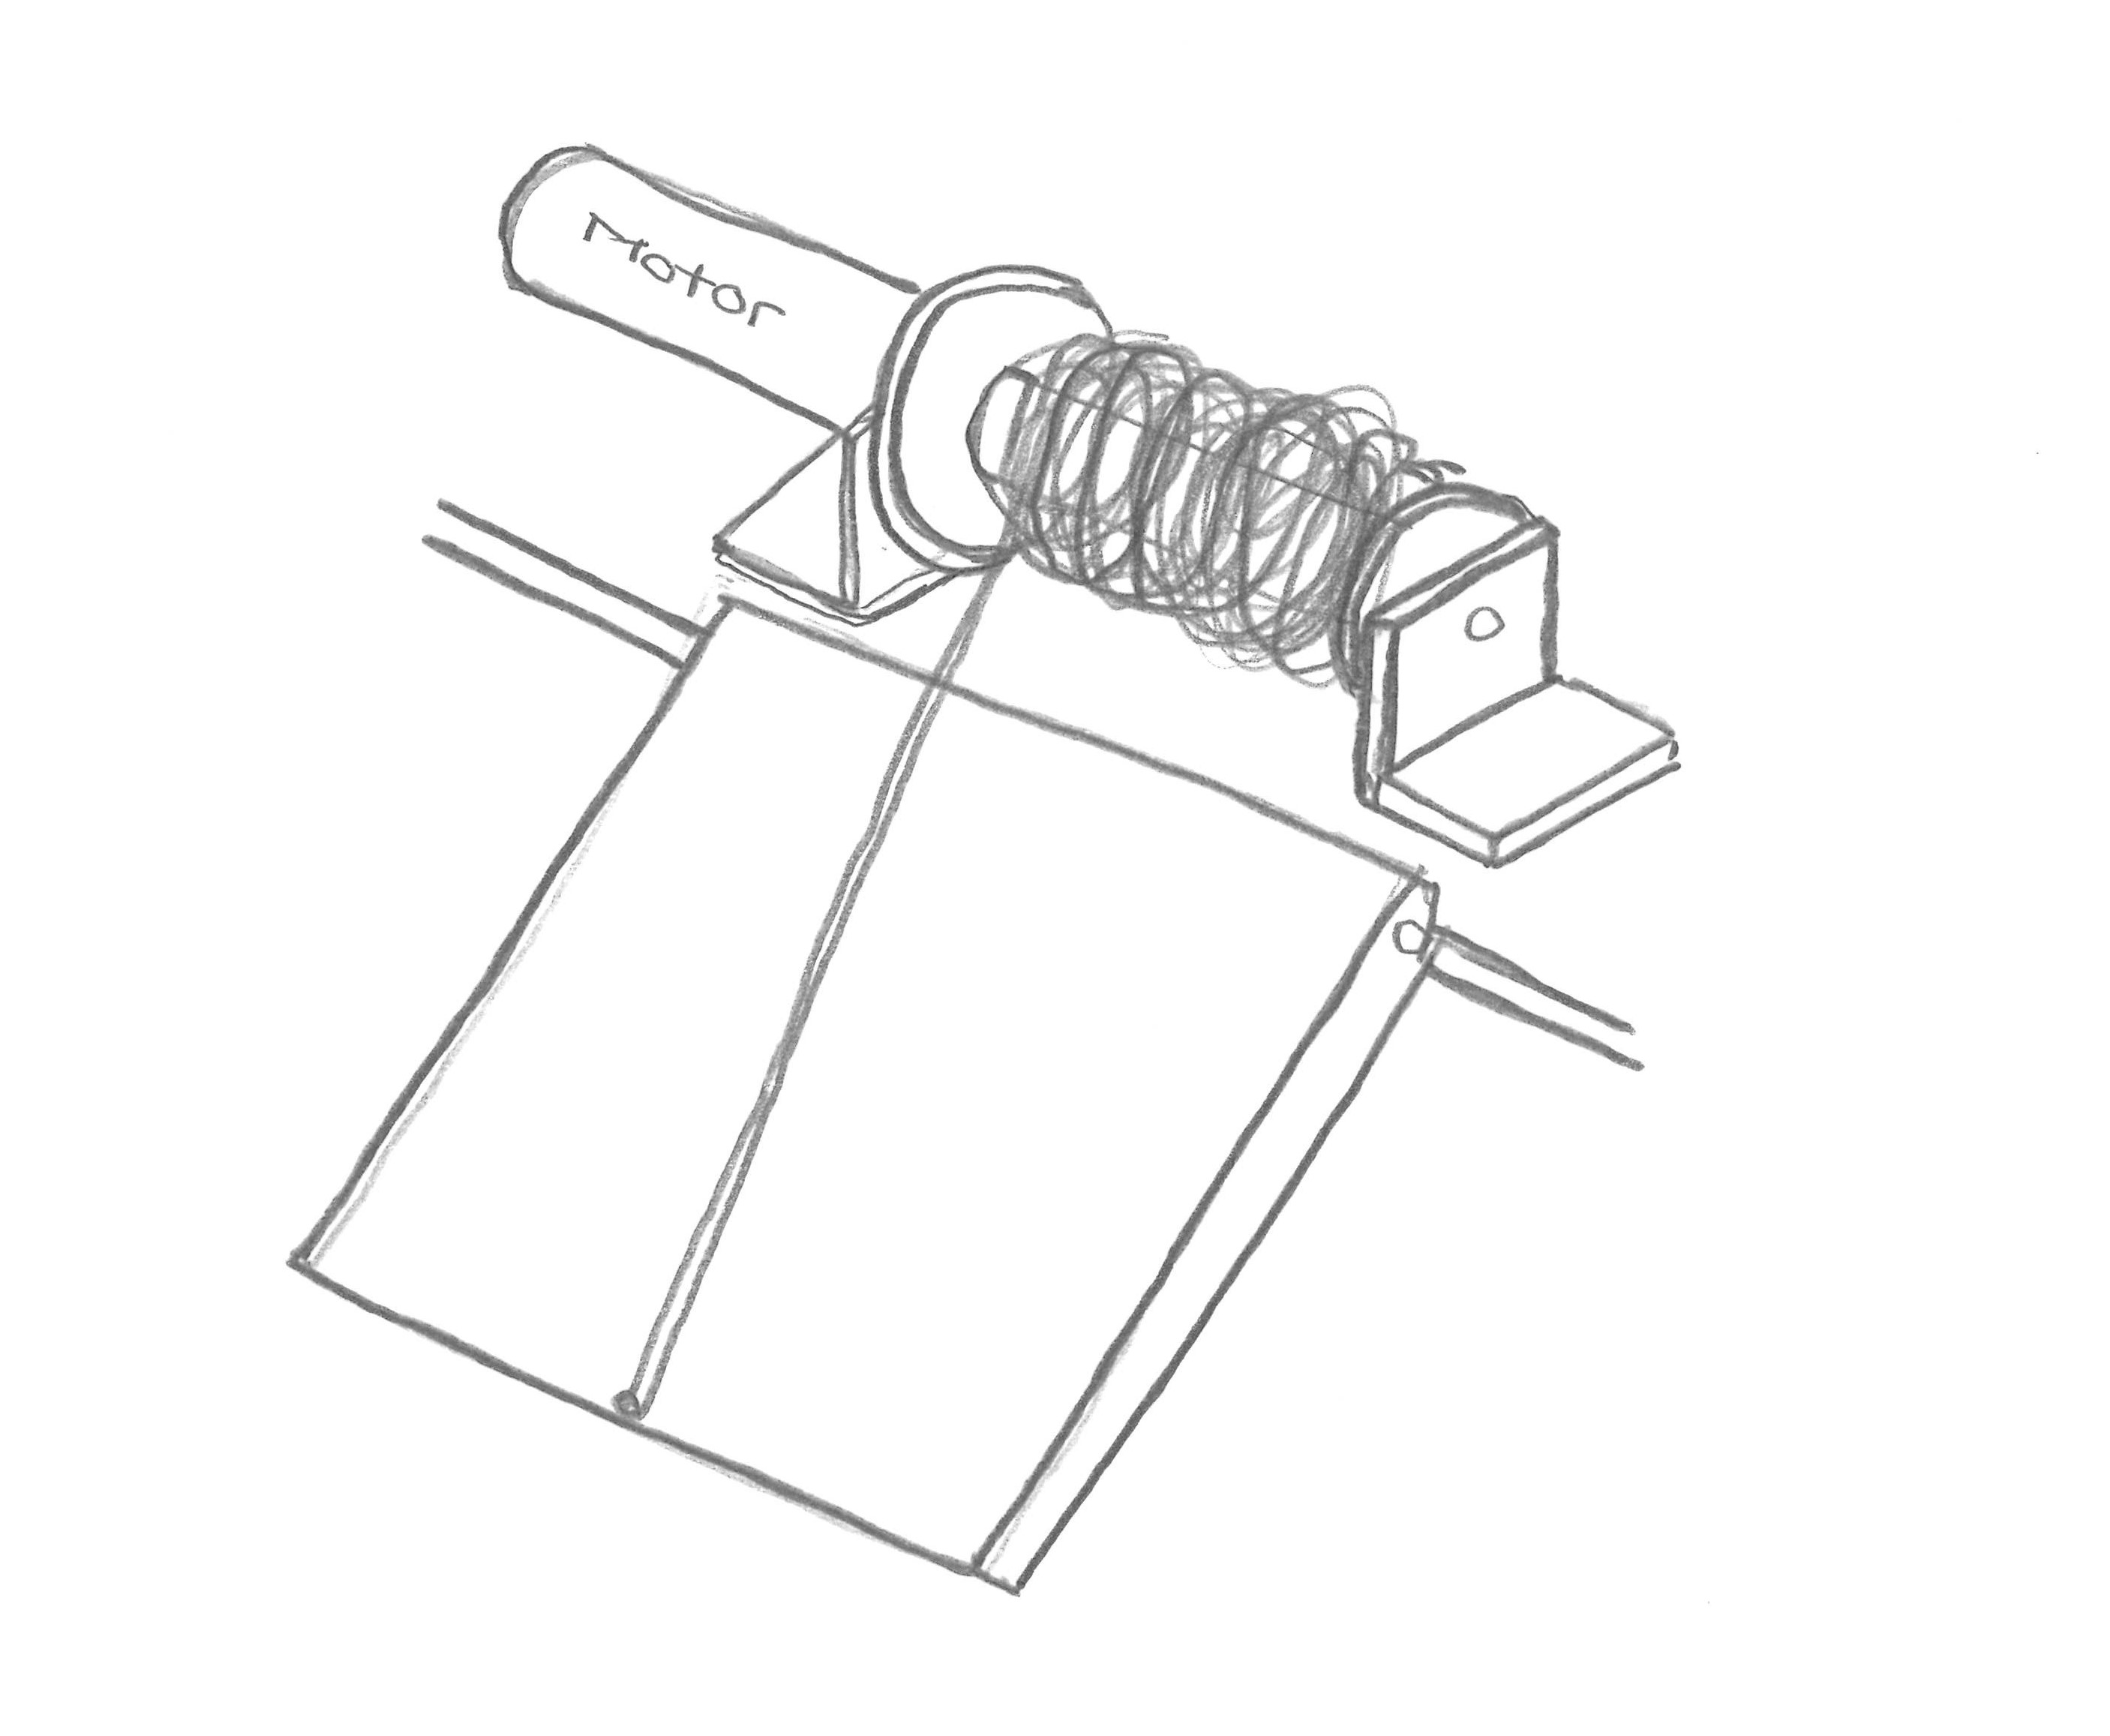
\includegraphics[width=0.7\textwidth]{Rampe}
    \caption{Lösungskonzept Rampe}
    \label{fig:rampe}
\end{figure}

\begin{flushleft}
    \begin{table}[h]
    \begin{tabular}{ | l | p{11cm} |}
    \hline
    \textbf{Problemstellung} & Würfeltransport: Verschieben \\ \hline
    \textbf{Disziplin} & Maschinentechnik \\ \hline
    \textbf{Lösungskonzept} &  Rampe mit Seilzug \\ \hline
    \textbf{Bewertung} &  \begin{itemize}
                            \item[+] Bewegung erfolgt nur auf einer Achse
                            \item[+] Einfachheit
                            \item[-] Mechanisch anspruchsvoller
                            \item[-] Grosser Bauraum
                          \end{itemize} \\ \hline
    \end{tabular}
    \caption{Konzeptbeurteilung: Würfeltransport mittels Rampe}
    \label{tab:konzept_wurfeltrransport_umschwenker}
\end{table}
\end{flushleft}
Für diese Konzeptlösung des Produktes wird anhand des Konzeptes des «Um- und Einschwenkers» bevorzugt. Die Rampe mit dem Seilzug ist mechanisch anspruchsvoller zu realisieren und wird somit nicht für die favorisierte Endlösung gewählt.

\textbf{Antrieb:}
Damit die Steuerung auch weiss wie viele Umdrehungen die Rädern gemacht, respektive wieviel Weg das Schienenfahrzeug zurückgelegt hat ist es wichtig einen schlupffreien Antriebsstrang zu haben. Für das gehen wir davon aus, dass die Räder nicht auf den Gleisen durchdrehen, dies wird erreicht in dem die Auflageflächen mit einem Antirutschmaterial beschichtet werden. In folgendem Abschnitt werden die zwei besten Lösungen anhan der Nutzwertanalyse (siehe Abbildung \ref{fig:antrieb}) für diese Problemstellung vorgestellt.

\begin{figure}[H] %Nutzwertanalyse Antrieb
    \centering
    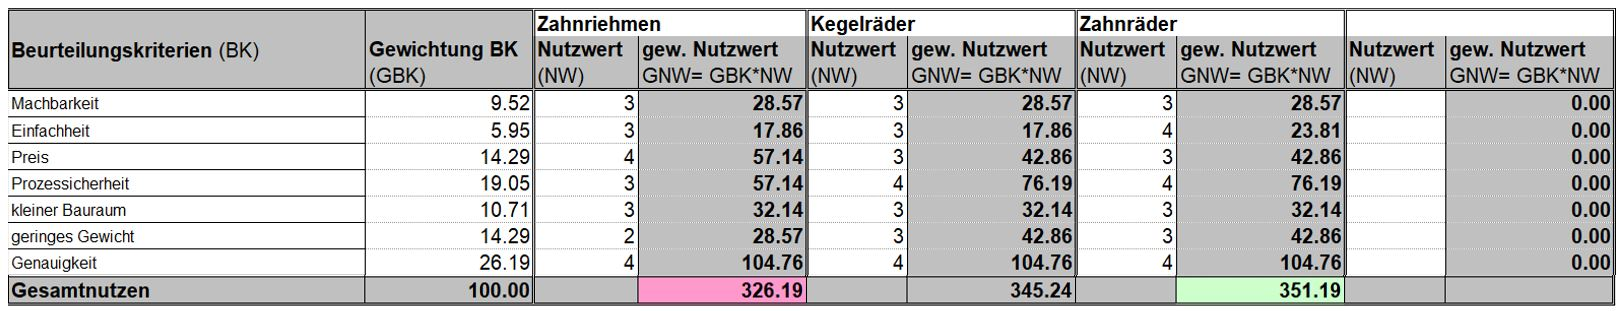
\includegraphics[width=1\textwidth]{Antriebsstrang}
    \caption{Nutzwertanalyse Antrieb}
    \label{fig:antrieb}
\end{figure}

\textbf{Zahnräder}
Um das Drehmoment auf die angetriebenen Räder zu bringen wird mittels Anordnung diverser Zahnräder gearbeitet. (siehe Tabelle \ref{tab:konzept_fahrwerk_zahnraeder})

\begin{flushleft}
    \begin{table}[h]
    \begin{tabular}{ | l | p{11cm} |}
    \hline
    \textbf{Problemstellung} & Antriebsstrang \\ \hline
    \textbf{Disziplin} & Maschinentechnik \\ \hline
    \textbf{Lösungskonzept} & Zahnräder \\ \hline
    \textbf{Bewertung} &  \begin{itemize}
                            \item[+] Direkte Kraftübertragung
                            \item[+] Schlupffrei
                            \item[+] Genauigkeit
                            \item[-] Komplexität
                            \item[-] Hohe Kosten
                          \end{itemize} \\ \hline
    \end{tabular}
    \caption{Konzeptbeurteilung: Antrieb mit Zahnräder}
    \label{tab:konzept_fahrwerk_zahnraeder}
\end{table}
\end{flushleft}

\textbf{Zahnriemen}
Der Antriebsstrang mit deinem Zahnriemen zu gestalten gib einem mehr Freiheit in der Positionierung des Antriebs mit dem Kompromiss, dass man einen langen Riemen bekommt, der durchhängen kann auf der nicht belasteten Seite. (siehe Tabelle \ref{tab:konzept_fahrwerk_zahnriemen})

\begin{flushleft}
    \begin{table}[h]
    \begin{tabular}{ | l | p{11cm} |}
    \hline
    \textbf{Problemstellung} & Dämpfung (für eine laufruhige Fahrt) \\ \hline
    \textbf{Disziplin} & Maschinentechnik \\ \hline
    \textbf{Lösungskonzept} & Zahnriemen \\ \hline
    \textbf{Bewertung} &  \begin{itemize}
                            \item[+] Direkte Kraftübertragung
                            \item[+] Freie Positionierung der Antriebs
                            \item[+] Schlupffrei
                            \item[-] Komplexität
                            \item[-] Hohe Kosten
                            \item[-] Durchhängen
                          \end{itemize} \\ \hline
    \end{tabular}
    \caption{Konzeptbeurteilung: Antrieb mit Zahnriemen}
    \label{tab:konzept_fahrwerk_zahnriemen}
\end{table}
\end{flushleft}

\end{document}